\themaM
\graphicspath{{../Ch22_Les_angles/Images/}}

\chapter{Angles et degrés}
\label{C13}


%%%%%%%%%%%%%%%%%%%%%%%%%%%%%%%%%%%%%%%%%
%%%%%%%%%%%%%%%%%%%%%%%%%%%%%%%%%%%%%%%%%
\begin{prerequis}[Connaissances et compétences associées]
   \begin{itemize}
      \item Identifier des angles dans une figure géométrique.
      \item Comparer des angles, en ayant ou non recours à leur mesure (par superposition, avec un calque).
      \item Reproduire un angle donné en utilisant un gabarit.
      \item Estimer qu’un angle est droit, aigu ou obtus.
      \item Utiliser l’équerre pour vérifier qu’un angle est droit, aigu ou obtus, ou pour construire un angle droit.
   \end{itemize}
\end{prerequis}

\vfill

\begin{debat}[Débat : angles et perspective]
   La {\bf perspective} est un ensemble de techniques destinées à représenter un objet ou une image en trois dimensions sur une surface plane. Il existe plusieurs sortes de perspectives, comme par exemple la perpective cavalière, la perspective isométrique, la perpective à point de fuite\dots{} Selon la perspective utilisée, on utilise des directions suivant des angles différents.
   \begin{center}
      \begin{pspicture}(0,-1)(4,3.5)
         \psframe(0,0)(1.5,1.5)
         \psline(0,1.5)(0.8,2.3)(2.3,2.3)(2.3,0.8)(1.5,0)
         \psline(1.5,1.5)(2.3,2.3)
         \psset{linestyle=dashed,linecolor=A1}
         \psline(0.8,2.3)(1.6,3.1)
         \psline(2.3,2.3)(3.1,3.1)
         \psline(2.3,0.8)(3.1,1.6)
         \rput(0.75,-0.75){\it cavalière}
      \end{pspicture}
      \begin{pspicture}(-2,-2.5)(2,2)
         \pspolygon(1.3;-30)(1.3;30)(1.3;90)(1.3;150)(1.3;-150)(1.3;-90)
         \psline(1.3;150)(0,0)(1.3;30)
         \psline(0,0)(1.3;-90)
        \psset{linestyle=dashed,linecolor=A1}
         \psline(1.3;150)(2.3;150)
         \psline(1.3;30)(2.3;30)
         \psline(1.3;-90)(2;-90)
         \rput(0,-2.25){\it isométrique}
      \end{pspicture}
      \begin{pspicture}(-1,-1)(3,3.5)
         \psframe(0,0)(1.5,1.5)
         \psline(0,1.5)(0.8,1.9)(1.9,1.9)(1.9,0.8)(1.5,0)
         \psline(1.5,1.5)(1.9,1.9)
         \psdot(3,3)
         \psset{linestyle=dashed,linecolor=A1}
         \psline(0.8,1.9)(3,3)
         \psline(1.9,1.9)(3,3)
         \psline(1.9,0.8)(3,3)
         \rput(0.75,-0.75){\it un point de fuite}
      \end{pspicture}
   \end{center}
   \bigskip
   \begin{cadre}[B2][F4]
      \begin{center}
         Vidéo : \href{https://www.youtube.com/watch?v=zCIxdOCQiZg}{\bf Comment dessiner des illusions d'optique 3D}, chaîne YouTube {\it Simple drawing tutorial}.
      \end{center}
   \end{cadre}
\end{debat}

\vfill

\textcolor{PartieGeometrie}{\sffamily\bfseries Cahier de compétences} : chapitre 8, exercices 1 ; 2 ; 5 ;  6 ; 9.


%%%%%%%%%%%%%%%%%%%%%%%%%%%%%%%%%%%%
%%%%%%%%%%%%%%%%%%%%%%%%%%%%%%%%%%%%
\activites

\begin{activite}[Une nouvelle unité de mesure]
   {\bf Objectif :} comparer des angles sans recours à la mesure ; découvrir le degré ; mesurer un angle donné.
   \begin{QCM}
      \partie[fabrication d'angles]
      {\it Partie à faire en binôme.}
         \begin{enumerate}
            \item 
            \begin{enumerate}
               \item Sur une feuille, construire deux \textbf{carrés} dont les mesures des côtés sont respectivement \ucm{4} et \ucm{7}.
               \item Découper ces carrés puis les plier en deux suivant une \textbf{diagonale} : on obtient pour chaque carré deux triangles identiques à découper.
               \begin{center}
                  {\psset{unit=0.7}
                  \begin{pspicture}(-0.5,-0.3)(4,3)
                     \psframe(0,0)(3,3)
                     \psline[linestyle=dashed](0,0)(3,3)
                     \rput(4,1.5){$\Longrightarrow$}
                  \end{pspicture}
                  \begin{pspicture}(0,-0.3)(4,3)
                     \pswedge[fillstyle=solid,fillcolor=G1,linecolor=G1](0,0){0.8}{0}{45}
                     \pswedge[fillstyle=solid,fillcolor=G1,linecolor=G1](3,3){0.8}{225}{-90}
                     \psframe[fillstyle=solid,fillcolor=B1,linecolor=B1](3,0)(2.5,0.5)
                     \pspolygon(0,0)(3,0)(3,3)
                  \end{pspicture}}
               \end{center}
            \end{enumerate}
            \item
            \begin{enumerate}
               \item Construire deux \textbf{triangles équilatéraux} dont les mesures des côtés sont respectivement de \ucm{5} et \ucm{7}.
               \item Découper ces triangles puis les plier en deux suivant une \textbf{hauteur} : on obtient pour chaque triangle deux triangles identiques à découper.
            \end{enumerate}
            \begin{center}
               {\psset{unit=0.7}
               \begin{pspicture}(0,0.3)(4.5,2.5)
                  \pspolygon(0,0)(3.5,0)(1.75,3.03)
                  \psline[linestyle=dashed](1.75,0)(1.75,3.03)
                  \rput(4,1.5){$\Longrightarrow$}
               \end{pspicture}
               \begin{pspicture}(-0.7,0.3)(2,2.5)
                 \pswedge[fillstyle=solid,fillcolor=J1,linecolor=J1](0,0){0.6}{0}{60}
                  \pswedge[fillstyle=solid,fillcolor=A1,linecolor=A1](1.75,3.03){0.7}{240}{-90}
                  \psframe[fillstyle=solid,fillcolor=B1,linecolor=B1](1.75,0)(1.25,0.5)
                  \pspolygon(0,0)(1.75,0)(1.75,3.03)
               \end{pspicture}}
            \end{center}
         \item Au total on obtient huit triangles, deux à deux identiques. Prendre chacun un triangle de chaque sorte. \bigskip
         \end{enumerate}

      \partie[classement des angles]
      \ \\ [-9mm]
         \begin{enumerate}
            \setcounter{enumi}{3}
            \item Colorier les trois angles de chaque triangle : combien d'angles différents obtient-on ? \pf \smallskip
            \item La taille des angles dépend-elle de la longueur des côtés ? \pf \smallskip
            \item Classer ces angles du plus grand au plus petit en les codant A, B, C et D (le plus grand est A) : \\ [1mm]
            \pf \\ [1mm]
            \textit{Ces différents angles sont appelés des \textbf{gabarits}.} \bigskip
         \end{enumerate}

      \partie[le degré]
         Le {\bf degré} est une unité de mesure d'angle. L'angle droit mesure \udeg{90}.
         \begin{enumerate}
            \setcounter{enumi}{6}
            \item À partir de l'assemblage de quels angles peut-on former l'angle A (deux possibilités) ? \\ [1mm]
            \pf \smallskip
            \item À partir de quels angles peut-on former l'angle B ? \pf \smallskip
            \item Sachant que l'angle A mesure \udeg{90}, retrouver la mesure des angles B, C et D. \\ [1mm]
               \pf \\ [1mm]
               \pf \\ [1mm]
               \pf \bigskip
         \end{enumerate}
    \end{QCM}
\end{activite}


%%%%%%%%%%%%%%%%%%%%%%%%%%%%%%%%%%%%%%%%%%%%%%%%%%%%%%%%%%%%%%%%%%%%%%%%
\cours 

%%%%%%%%%%%%%%%%%%%%%%%%%%%%%%%
\section{Les angles}

\begin{definition}
   Un \textbf{angle} est une portion du plan délimitée par deux droites.
\end{definition}

\begin{pspicture}(-6,-0.3)(4,2.7)
   {\psset{yunit=0.6}
   \small
   \rput(0,-0.3){A}
   \rput(4,3.6){B}
   \rput(0,2.35){C}
   \rput(4,0.4){D}
   \rput(1.4,1){O}
   \psline(0,0)(4,4)
   \psline(0,2)(4,0)
   \psarc[linecolor=A1](1.4,1.4){1}{-20}{30}
   \psline[linecolor=B2]{->}(-1,1.1)(1.3,1.3)
   \rput(-1.8,1.3){\textcolor{B2}{sommet}}
   \rput(3.5,1.7){\textcolor{A1}{angle $\widehat{BOD}$}}}
\end{pspicture}

En général, on marque l'angle considéré par un arc de cercle. Pour nommer un angle, il suffit de connaître son sommet et un point de chacun de ses côtés.

\begin{exemple}
   \begin{pspicture}(-1,-0.5)(3,2)
      \psset{unit=1.2}
      \pspolygon(0,0)(3,0)(3,1.5)
      \rput(0,-0.3){A}
      \rput(3,-0.3){B}
      \rput(3,1.8){C}
      \psarc[linecolor=A1,doubleline=true](0,0){0.7}{0}{27}
      \psarc[linecolor=J1,linestyle=dashed](3,0){0.5}{90}{180}
      \psarc[linecolor=B1](3,1.5){0.5}{205}{270}
   \end{pspicture}
   \correction
   Dans le triangle (trois angles) ABC, on a les angles :
   \begin{itemize}
      \item \textcolor{A1}{$\widehat{BAC} =\widehat{CAB}$} ;
      \item \textcolor{J1}{$\widehat{ABC} =\widehat{CBA}$} ;
      \item \textcolor{B1}{$\widehat{BCA} =\widehat{ACB}$}.
   \end{itemize}
\end{exemple}


%%%%%%%%%%%%%%%%%%%%%%%%%%%%%%%%%%%
\section{Le degré}

\begin{definition}
   Pour mesurer l'ouverture d'un angle, on utilise au collège le {\bf degré} noté \degre.
\end{definition}

\begin{minipage}{7cm}
   {\psset{unit=0.7}
   \begin{pspicture}(-5,-3.5)(4,4)
      \pscircle(0,0){3}
      \multido{\n=0+10}{36}{\psline[linecolor=lightgray](0;\n)(3.1;\n)\rput(3.5;\n){\tiny\n}}  
      \psline(-3,0)(3,0)
      \psline(0,-3)(0,3)  
   \end{pspicture}}
\end{minipage}
\begin{minipage}{8cm}
   L'angle droit mesure \udeg{90}. \\
   Un angle plat, c'est deux angles droits, soit \udeg{180}. \\
   Un tour entier, c'est quatre angles droits, soit \udeg{360}.
\end{minipage}

\begin{minipage}{4.5cm}
   On peut classer les angles \\
   selon leur mesure en degrés : 
\end{minipage}
\begin{minipage}{10cm}
   \begin{center}
      \begin{pspicture}(-4.5,-0.5)(3,2.5)
         \rput(0,-0.3){0}
         \rput(4,0){angle nul : 0\degre}
         \pswedge[fillstyle=solid,fillcolor=B2,linecolor=B2](0,0){1.5}{0}{90}
         \rput(2.5,1.5){\parbox{2cm}{\textcolor{B2}{angle aigu : \\ 0\degre < \pswedge[fillstyle=solid,fillcolor=B2,linecolor=B2](0.2,0){0.3}{0}{90} \qquad\, < 90\degre}}}
         \pswedge[fillstyle=solid,fillcolor=A1,linecolor=A1](0,0){1.5}{90}{180}
         \rput(-2.5,1.5){\parbox{2.5cm}{\textcolor{A1}{angle obtus : \\ 90\degre < \pswedge[fillstyle=solid,fillcolor=A1,linecolor=A1](0.4,0){0.3}{90}{180} \quad\;\; < 180\degre}}}
         \rput(0,2.5){angle droit : 90\degre}
         \rput(-4,0){angle plat : 180\degre}
         \psline(-2.5,0)(2.5,0)
         \psline(0,2)
      \end{pspicture}
   \end{center}
\end{minipage}

\begin{remarque}
   pour mesurer un angle, on utilise un {\bf rapporteur}, son utilisation sera vue dans le chapitre 28. Ici, on utilisera l'équerre pour savoir si un angle est aigu, droit ou obtus.
\end{remarque}


%%%%%%%%%%%%%%%%%%%%%%%%%%%%%%%%
%%%%%%%%%%%%%%%%%%%%%%%%%%%%%%%%
\exercicesbase

\begin{colonne*exercice}

\serie{Nom des angles } %%%%%%%%%

\begin{exercice} %1
   Utiliser les figures ci-dessous pour compléter le tableau.
   \begin{center}
      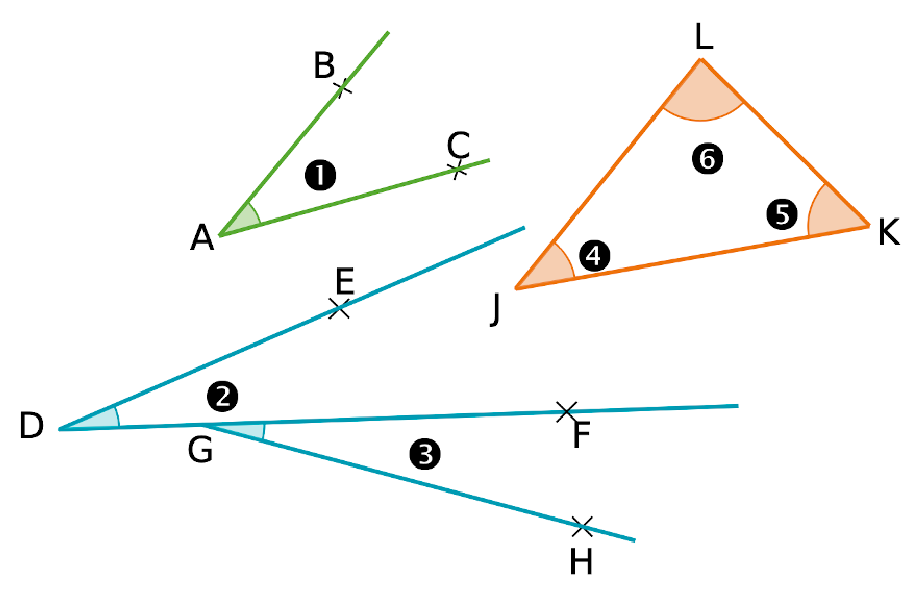
\includegraphics[width=8cm]{noms_angles} \\ [5mm]
      {\hautab{1.5}
      \begin{Ltableau}{0.9\linewidth}{4}{c}
         \hline
         Angle & nom & sommet & côtés \\
         \hline
         1 & & & \\
         \hline
         2 & & & \\
         \hline
         3 & & & \\
         \hline
         4 & & & \\
         \hline
         5 & & & \\
         \hline
      \end{Ltableau}}
   \end{center}
\end{exercice}

\medskip

\begin{exercice} %2
   Sur la figure suivante : \\
   \begin{center}
      \begin{pspicture}(-0.3,-0.3)(8,4)
         \pstGeonode[PointSymbol=none,PosAngle={90,110,90,100,120,90}](1,4){A}(3.5,4){B}(7,4){C}(3,2.8){D}(2.5,1.3){E}(4,2.2){F}
         \pstLineAB[nodesepA=-1,nodesepB=-1]{A}{C}
         \pstLineAB[nodesepA=-0.8,nodesepB=-1.3]{B}{E}
         \pstLineAB[nodesepA=-1,nodesepB=-3]{A}{F}
         \pstLineAB[nodesepA=-1,nodesepB=-2]{C}{E}
         \rput(6.5,1.1){$G$}
         \rput(0.4,3.6){$H$}
         \rput(1,0.8){$I$}
         \rput(2.6,0.3){$J$}
      \end{pspicture}
      \begin{enumerate}
         \item Colorier en vert l'angle $\widehat{ADB}$.
         \item Colorier en rouge l'angle $\widehat{CFA}$.
         \item Colorier en noir l'angle $\widehat{DEF}$.
         \item Colorier en bleu l'angle $\widehat{BCF}$.
         \item Donner d'autres noms à l'angle $\widehat{DFE}$.
         \item Donner d'autres noms à l'angle $\widehat{BEC}$.
      \end{enumerate}
   \end{center}
\end{exercice}

\serie{Types d'angles} %%%

\begin{exercice} %3
   Pour chaque cas, donner la nature de l'angle (aigu, obtus, droit ou plat).
   \begin{colenumerate}{2}
      \item \udeg{27} \pf \smallskip
      \item \udeg{32} \pf \smallskip
      \item \udeg{12,3} \pf \smallskip
      \item \udeg{179,9} \pf \smallskip
      \item \udeg{90} \pf \smallskip
      \item \udeg{80} \pf \medskip
      \item \udeg{1} \pf
      \item \udeg{180} \pf
      \item \udeg{154} \pf
      \item \, \udeg{93,90} \pf
      \item \, \udeg{89,999} \pf
      \item \, \udeg{0} \pf
   \end{colenumerate}
\end{exercice}

\begin{exercice} %4
   Marquer les angles aigus d'un arc rouge, les angles obtus d'un arc bleu et les angles droits avec un carré vert.
   \begin{center}
         \begin{pspicture}(0,1)(8,7.5)
         \pspolygon(1,2)(1,7)(7,7)(7,6)(4,5)(2,6)(2,4)(4,2)(5,4)(6,5)(5,1)
      \end{pspicture}
   \end{center}
\end{exercice}

\begin{exercice} %5
   Pour chaque chiffre, marquer tous les angles plus petits qu'un angle plat puis les dénombrer. \\
   Que remarque-t-on ? \medskip
   \begin{center}
      {\psset{unit=0.5}
      \begin{pspicture}(0,0)(3,4)
         \psellipse(1,2)(1,2)
      \end{pspicture}
      \begin{pspicture}(0,0)(3,4)
         \psline(0,2)(2,4)(2,0)
      \end{pspicture}
      \begin{pspicture}(0,0)(3,4)
         \psline(0,4)(2,4)(0,0)(2,0)
      \end{pspicture}
      \begin{pspicture}(0,0)(3,4)
         \psline(0,4)(2,4)(0,2)(2,0)(0,0)
      \end{pspicture}
      \begin{pspicture}(0,0)(2,4)
         \psline(2,0)(2,4)(0,2)(2,2)
      \end{pspicture} \\ [8mm]
      \begin{pspicture}(0,0)(3,4)
         \psline(2,4)(0,4)(0,2)(2,2)(2,0)(0,0)(0,0.5)
      \end{pspicture}
      \begin{pspicture}(0,0)(3,4)
         \psline(2,4)(0,4)(0,2)(2,2)(2,0)(0,0)(0,2)
      \end{pspicture}
      \begin{pspicture}(0,0)(3,4)
         \psline(0,4)(2,4)(0.5,0)
         \psline(0.5,2)(2,2)
         \psline(0,0)(1,0)
      \end{pspicture}
      \begin{pspicture}(0,0)(3,4)
         \psframe(0,0)(2,4)
         \psline(0,2)(2,2)
      \end{pspicture}
      \begin{pspicture}(0,0)(2,4)
         \psline(2.5,2)(0,2)(0,4)(2,4)(2,0)(0,0)(0,0.5)
      \end{pspicture}}
   \end{center}
\end{exercice}

\end{colonne*exercice}


%%%%%%%%%%%%%%%%%%%%%%%%%%%%%%%%%%%%
%%%%%%%%%%%%%%%%%%%%%%%%%%%%%%%%%%%%
\Recreation

   \enigme[Le triangle de Penrose]
      \partie[une figure impossible]
         Le {\bf triangle de Penrose}, aussi appelé tripoutre ou tribarre est un triangle impossible à construire physiquement en 3D mais facilement modélisable en 2D. Il a été conçu par le physicien et mathématicien britannique {\bf Roger Penrose} (né à Colchester en 1931) dans les années 1950.
         \begin{enumerate}
            \item Observer le triangle de Penrose et en particulier ses angles sur ce quadrillage à maille triangulaire (aussi appelé isométrique en raison de l'égalité de longueur de tous ses côtés). Pourquoi est-il impossible à construire ?
            \item Le reproduire sur le quadrillage juste à droite, puis le colorier. \\
         \end{enumerate}
         \begin{pspicture*}(0,2)(17,11)
            \pstVerb{gsave [0.866 0.5 0 1 0 -400] concat }
            {\psset{linewidth=0.3pt,linecolor=black!40}
               \multido{\iA=-0+1,\iB=-10+1,\iC=-25+1}{40}{
                  \psline(\iA,-4)(\iA,20)
                  \psline(-5,\iB)(20,\iB)
                  \rput(0,\iC){\psline(0,0)(!\iA\space abs dup add dup )}}}
            \pspolygon[fillstyle=solid,fillcolor=PartieStatistique](2,2)(1,2)(1,8)(6,8)(5,7)(2,7)
            \pspolygon[fillstyle=solid,fillcolor=PartieStatistique!66](2,2)(2,7)(3,7)(3,4)(8,9)(8,8)
            \pspolygon[fillstyle=solid,fillcolor=PartieStatistique!33](3,4)(3,5)(6,8)(1,8)(2,9)(8,9)
            \pstVerb{grestore}
         \end{pspicture*}

      \partie[d'autres curiosités]
      \ \\ [-10mm]
         \begin{enumerate}
            \item Le jeu {\bf Monument Valley} est un jeu de réflexion en perspective isométrique qui se passe dans un décor composé de structures aux formes géométriques impossibles basées sur ce triangle.
            \item {\bf An impossible triangle sculpture in Perth.} \\
               In 1997, a new landmark has been created for Perth, in a unique collaboration between a leading WA artist Brian McKay and architect Ahmad Abas. Destined to become a bold icon for Perth, the \og Impossible Triangle \fg{} has been erected in Claisebrook Square, East Perth. The sculpture is 13.5 meters height and the design striations on the polished aluminium reflects both sunlight and artificial lighting. The view of the triangle depends on where it is observed from. \hfill {\footnotesize\it Source : https://im-possible.info/english/}
            \end{enumerate}
            \begin{center}
               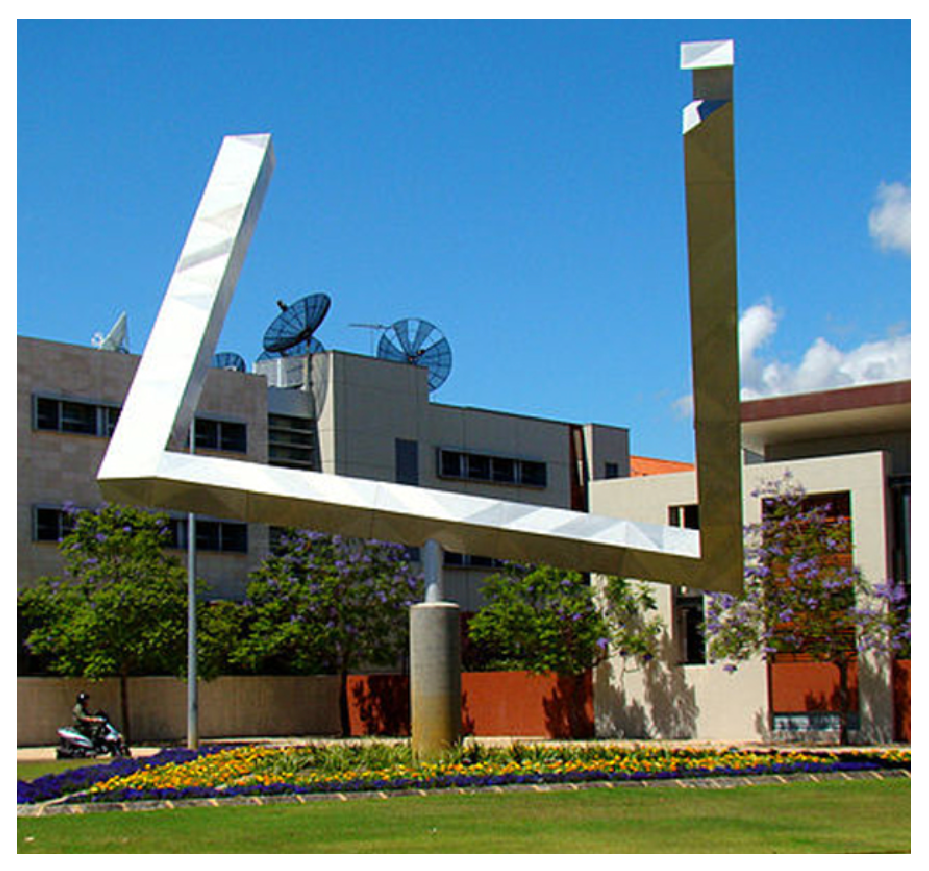
\includegraphics[height=3.5cm]{Penrose1} \qquad 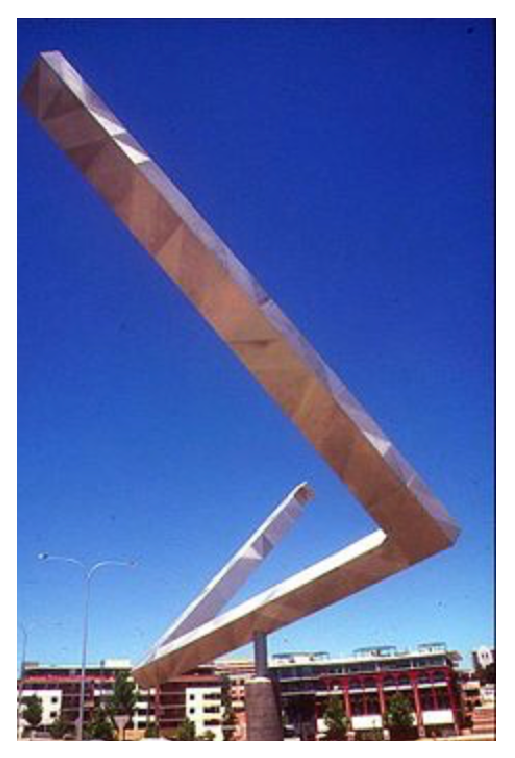
\includegraphics[height=3.5cm]{Penrose2} \qquad 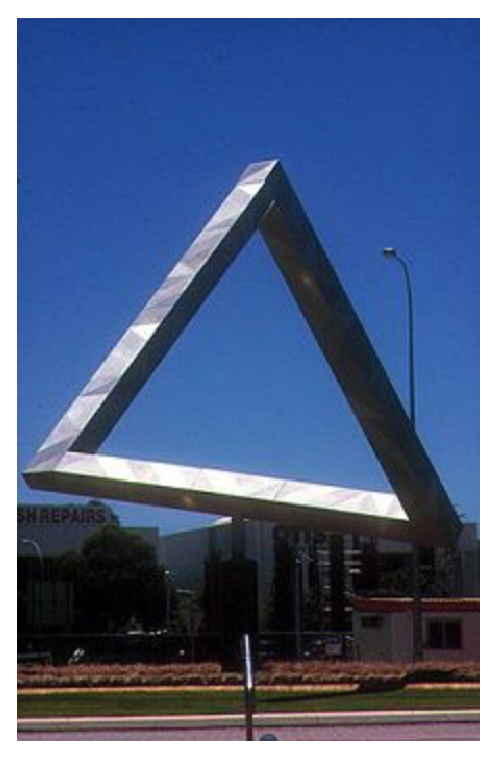
\includegraphics[height=3.5cm]{Penrose3}
            \end{center}

